 
%----------------------------------------------------------------------------------------
%	PACKAGES AND THEMES
%----------------------------------------------------------------------------------------
\documentclass[aspectratio=169,xcolor=dvipsnames,noframenumbering]{beamer}

\usetheme{SimplePlusAIC}


\renewcommand\emph[1]{{\color{darkred} #1}}
\newcommand\myemph[1]{{\color{darkred} #1}}
\newcommand\platz{\vspace{.7cm}}
\newcommand\tabb{\hspace{.75cm}}

\usepackage{mathrsfs}
%\usepackage{ulem}

\usepackage{color}
\definecolor{navy}{RGB}{0,0,205}
\definecolor{NavyBlue}{RGB}{0,0,205}
\definecolor{darkred}{RGB}{178,34,34}
\definecolor{darkblue}{RGB}{0,10,230}
\definecolor{green}{RGB}{20,180,20}
\definecolor{titleblue}{rgb}{0,0,0.3}
\definecolor{mediumblue}{rgb}{0.5,0.5,1}
\definecolor{lightblue}{cmyk}{0.2,0.1,0,0}
\definecolor{darkgreen}{rgb}{0.0,0.5,0}

\newcommand{\mnred}[1]{{\color{red}#1}}
\newcommand{\mred}[1]{{\color{darkred}#1}}
\newcommand{\mgreen}[1]{{\color{green}#1}}

\newcommand{\scriptgray}[1]{{ \scriptsize \color{gray}#1}}

\DeclareMathOperator{\lcm}{lcm}

\newcommand{\toright}[1]{{ \hfill{\scriptgray{#1}}}}

\newcommand{\cone}{\operatorname{cone}}
\newcommand{\intcone}{\operatorname{intcone}}
\newcommand{\poly}{\operatorname{poly}}
\newcommand{\rank}{\operatorname{Rank}}
\newcommand{\setR}{\mathbb{R}}
\newcommand{\setZ}{\mathbb{Z}}
\newcommand{\setQ}{\mathbb{Q}}
\newcommand{\R}{\mathbb{R}}
\newcommand{\Z}{\mathbb{Z}}
\newcommand{\Q}{\mathbb{Q}}


\renewcommand\geq{\geqslant}
\usepackage{hyperref}
\usepackage{graphicx} % Allows including images
\usepackage{booktabs} % Allows the use of \toprule, \midrule and  \bottomrule in tables  
\usepackage{svg} %allows using svg figures



\usepackage{tikz}
\usetikzlibrary{arrows.meta,patterns}
\usetikzlibrary{ipe} % ipe compatibility library

\usepackage{../tikzit}
\input{../TIKZ/digraph.tikzstyles}



\usepackage[utf8]{inputenc} 
\usepackage{utf8math}


\usepackage[round]{natbib}   % omit 'round' option if you prefer square brackets
\bibliographystyle{plainnat}


\usepackage{verbatim}
\usetikzlibrary{arrows,shapes} 
\usepackage{makecell}
\usepackage{amsmath}
\usepackage{mathtools}
\usepackage{caption}
\usepackage{subcaption}
\newcommand*{\defeq}{\stackrel{\text{def}}{=}}
\newcommand{\N}{\mathbb{N}}


\newcommand{\E}{\mathbb{E}}
\newcommand{\B}{\mathcal{B}}
\newcommand{\C}{\mathcal{C}}
\newcommand{\D}{\mathcal{D}}
\newcommand{\Polyhedre}{\mathcal{P}}
\newcommand{\Set}{\mathcal{S}}
\newcommand{\Lcone}{\mathbb{L}}
\newcommand{\Lapprox}{\mathcal{L}}
\newcommand{\epl}{\varepsilon}
\DeclarePairedDelimiter\ceil{\lceil}{\rceil}
\DeclarePairedDelimiter\floor{\lfloor}{\rfloor}
\makeatletter
\DeclareRobustCommand*{\bfseries}{%
  \not@math@alphabet\bfseries\mathbf
  \fontseries\bfdefault\selectfont
  \boldmath
}
\makeatother 
\makeatletter
\newcommand{\Pause}[1][]{\unless\ifmeasuring@\relax
\pause[#1]%
\fi}
\makeatother
\tikzset{hide on/.code={\only<#1>{\color{white}}}}
\tikzstyle{flowchart} = [rectangle, rounded corners, minimum width=3cm, minimum height=1cm,text centered, draw=black]
%Select the Epilogue font (requires luaLatex or XeLaTex compilers)

\usepackage{tgadventor}
\renewcommand*\familydefault{\sfdefault} %% Only if the base font of the document is to be sans serif
\usepackage[T1]{fontenc}





    
%----------------------------------------------------------------------------------------
%	TITLE PAGE
%----------------------------------------------------------------------------------------

\title{Discrete Optimization}
\subtitle{MATH-261}

\author[Eisenbrand]{Fritz Eisenbrand}

 
 

\date{}
%----------------------------------------------------------------------------------------
%	PRESENTATION SLIDES
%----------------------------------------------------------------------------------------


%\includeonly{lecture02}
\begin{document}

\begin{frame}[plain]
    % Print the title page as the first slide
    \titlepage
\end{frame}

\pagestyle{empty} 

\begin{frame}{Information on} 

    \begin{columns}
      \begin{column}{.5\textwidth}
        \begin{itemize}
        \item Content
         \item Exercices and exam
         \item Contact and forum
         \end{itemize}
       \end{column}
       \begin{column}{.5\textwidth}
         %  \begin{itemize}
         % \item Contenue du cours
         % \item Exercices et examen 
         % \item Contact et forum
         % \end{itemize}
       \end{column}
       
    \end{columns}
      
     % \end{alertblock}
     %      \begin{center}
     %   \input{}       
     % \end{center}    
    
  
  \end{frame}
   



   \begin{frame}

     \begin{columns}
       \begin{column}{0.4\textwidth }                 
     \frametitle{Assistants}
     Main assistants:
     \begin{itemize}
     \item Neta Singer
     \item Jiaye Wei
     \end{itemize}

     \bigskip 
     
     Student assistants 
     \begin{itemize}
     \item Sayantan Biswas
     \item Mehdi Aziz Jelassi 
     \end{itemize}
   \end{column}
   \begin{column}{0.4\textwidth }
   \end{column}
 \end{columns}
\end{frame}

   \begin{frame}{Content}
   
     \begin{enumerate}
     \item    Linear optimization problems 
     \item    Convex geometry: Polyhedra, convex sets, Farkas' Lemma 
     \item    The simplex algorithm
     \item     Duality, Zero sum games: Von Neumann's theorem 
     \item     Analysis of algorithms: Gaussian elimination and running time of simplex algorithm
\item     Ellipsoid method and convex optimization problems
   \end{enumerate}

   \end{frame}

   \begin{frame}{Course notes (polycopié)}

     \bigskip 
     
     Can be found on moodle page

     \bigskip 
     Regularly updated 

     \bigskip 

     More content than covered in this course    
     
   \end{frame}
   


   \begin{frame}
     \frametitle{Exercises}

     \begin{itemize}
     \item One set each week 
     \item First problem sheet online today (Discussed Feb 25) 
     \item Problem set week $n$:
       \begin{itemize}
       \item Online after lecture
       \item Discussed in exercise session of following week 
       \end{itemize}
     \end{itemize}     
   \end{frame}

   \begin{frame}
     \frametitle{Exam}

     \begin{itemize}
     \item 2-3 open questions 
     \item $∼$ 4 questions  \myemph{multiple choice} 
     \item  $∼$ 8 questions \myemph{true/false}     
     \end{itemize}

   \end{frame}


   \begin{frame}{Contact/communication}

     \begin{itemize}
     \item Questions, comments: \myemph{Forum}
     \item \myemph{Format questions in latex!} 
     \item Please do not send me e-mails !
     \item Office hours: Wednesday 16:00 - 17:00 
     \item  schedule time-slot with: e-mail  {\tt pauline.bataillard@epfl.ch  }
     \end{itemize}
     
   \end{frame}


   

%%% Local Variables:
%%% mode: latex
%%% TeX-master: "Slides"
%%% End:

\begin{frame}{Optimization problems}

    \begin{columns}
      \begin{column}{.5\textwidth}
        \emph{Optimization problem}  is pair $(ℱ,f)$

        \medskip 

        \begin{itemize}
        \item $ℱ$ is set of \emph{feasible solutions}
        \item $f: ℱ ⟶ ℝ$  \emph{objective} or \emph{cost function}.
        \end{itemize}

        \bigskip
        
Task: Find  $x ∈ ℱ$ s.t. 
\begin{displaymath}
  f(x) ≥ f(y) \text{ holds for all } y ∈ ℱ 
\end{displaymath}
      \end{column}
      \begin{column}{.5\textwidth}
        Such  $x∈ ℱ$  is  \emph{optimal solution}

        \bigskip 
        We also write 
\begin{displaymath}
  \max \{ c(x) : x ∈ ℱ\}. 
\end{displaymath}
      \end{column}       
    \end{columns}
  \end{frame}


  \begin{frame}{Minimization}

    \begin{columns}[t]
      \begin{column}[t]{.5\textwidth}
        If  minimize $f(x)$, i.e.

        \bigskip 
        find  $x ∈ ℱ$ with  
\begin{displaymath}
  f(x) ≤ f(y) \text{ for all } y ∈ ℱ 
\end{displaymath}
        
      \end{column}
      \begin{column}{.5\textwidth}
        This is optimization problem $(ℱ,-f)$ since


        \bigskip

        \begin{displaymath}
          \begin{array}{l}
            -f(x) ≥ - f(y) \text{ for all } y ∈ ℱ \\[1ex] \text{ if and only if } \\[1ex] f(x) ≤ f(y) \text{ for all } y ∈ ℱ.
          \end{array}
        \end{displaymath}
      \end{column}       
    \end{columns}
  \end{frame}

\begin{frame}{Example: Maximizing quadratic form over sphere}

    \begin{columns}[t]
      \begin{column}{.5\textwidth}
        Max. $ x^T A x$ over domain

        
        $$S^{(d-1)} = \{ x ∈ ℝ^d : \|x\| = 1 \} ⊆ ℝ^d$$

        \bigskip 
       $A ∈ ℝ^{d×d}$  symmetric
        
      \end{column}
      \begin{column}{.5\textwidth}
        $ℱ = S^{(d-1)}$

        \medskip 
        $f(x) = x^T A x$

        \bigskip 
  \begin{displaymath}
    \max\left\{ x^T A x : x ∈S^{(d-1)} \right\}. 
  \end{displaymath}
      \end{column}       
    \end{columns}
  \end{frame}


\begin{frame}{Example: Minimizing quadratic form over sphere}

    \begin{columns}[t]
      \begin{column}{.5\textwidth}
        Min $ x^T A x$ over domain

        
        $$S^{(d-1)} = \{ x ∈ ℝ^d : \|x\| = 1 \} ⊆ ℝ^d$$

        \bigskip 
       $A ∈ ℝ^{d×d}$  symmetric
        
      \end{column}
      \begin{column}{.5\textwidth}
        $ℱ = S^{(d-1)}$

        \medskip 
        $f(x) = x^T (-A) x$

        \bigskip 
  \begin{displaymath}
    \min\left\{ x^T A x : x ∈S^{(d-1)} \right\}. 
  \end{displaymath}
      \end{column}       
    \end{columns}
  \end{frame}



  

\begin{frame}{Example: Shortest path in directed graph}

    \begin{columns}[t]
      \begin{column}{.5\textwidth}        
       Directed graph: Tuple  $G = (V,A)$

       \medskip
       $V$: finite set of \emph{vertices}

       \medskip
       $A ⊆ V ×V$: \emph{arcs}

       \medskip

       $w: A ⟶ ℝ$: \emph{weights}

       \medskip 
       \emph{Simple path}:  $P = v_1,v_2,\dots,v_k$  s.t.

       \smallskip 
       $v_i$ distinct and

       \smallskip 
       $(v_i,v_{i+1}) ∈A$  $i ∈ \{1,\dots,k-1\}$ 

       \medskip
\emph{length}: 
    $ℓ(P) = ∑_{i=1}^{k-1 } w(v_i,v_{i+1})$ 
  \end{column}
  \begin{column}{.5\textwidth}
    
    
    \begin{tikzpicture}
	\begin{pgfonlayer}{nodelayer}
		\node [style=new style 0] (0) at (0, 5) {$a$};
		\node [style=new style 0] (1) at (2, 3) {$b$};
		\node [style=new style 0] (2) at (0, 2) {$d$};
		\node [style=new style 0] (3) at (2, 1) {$e$};
		\node [style=new style 0] (4) at (-1, 0) {$f$};
		\node [style=new style 0] (5) at (-2, 3) {$c$};
		\node [style=none] (6) at (1.25, 4.25) {$1$};
		\node [style=none] (7) at (-1.25, 4.25) {$3$};
		\node [style=none] (8) at (-0.25, 3.25) {$1$};
		\node [style=none] (9) at (-1.25, 2.25) {};
		\node [style=none] (10) at (-1.25, 2.25) {$0$};
		\node [style=none] (11) at (0.75, 1.5) {$2$};
		\node [style=none] (12) at (0.75, 0.25) {$1$};
		\node [style=none] (13) at (-1.75, 1.25) {$1$};
		\node [style=none] (14) at (2.25, 2.25) {$0$};
	\end{pgfonlayer}
	\begin{pgfonlayer}{edgelayer}
		\draw [style=edge] (0) to (1);
		\draw [style=edge] (0) to (2);
		\draw [style=edge] (1) to (3);
		\draw [style=edge] (2) to (3);
		\draw [style=edge] (3) to (4);
		\draw [style=edge] (0) to (5);
		\draw [style=edge] (5) to (4);
		\draw [style=edge] (5) to (2);
	\end{pgfonlayer}
\end{tikzpicture}
   
    

  \end{column}       
\end{columns}
\end{frame}


\begin{frame}{Shortest path}

    \begin{columns}
      \begin{column}{.5\textwidth}
        Given: $G = (V,A)$

        \medskip
        $w: A ⟶ ℝ$

        \medskip
        $s,t ∈ V$ 


        \bigskip
        Shortest path problem:

        \medskip 
        $(ℱ,f)$ 
      \end{column}
      \begin{column}{.5\textwidth}

      \end{column}       
    \end{columns}
  \end{frame}


\begin{frame}{Linear Programming}

    \begin{columns}
      \begin{column}{.5\textwidth}
        $
          ℱ = \{ x ∈ ℝ^n : Ax ≤ b\}, 
          $

        \medskip   
        $A ∈ ℝ^{m ×n}$ $b ∈ ℝ^{m}$

        \bigskip 
        $f: ℝ^n ⟶ℝ$    \emph{linear}, i.e.,

        \medskip 
        $f(x) = c^Tx$ for $c ∈ ℝ^n$ 

      \end{column}
      \begin{column}{.5\textwidth}

      \end{column}       
    \end{columns}
  \end{frame}


\begin{frame}{Linear programming: Example}

    \begin{columns}
      \begin{column}{.5\textwidth}    
  \begin{displaymath}
    A =
    \begin{pmatrix}
      -1 & 1 \\
      1 & 1 \\
      0 & -1 
    \end{pmatrix}
  \end{displaymath}
  \begin{displaymath}
    b =
    \begin{pmatrix}
      1 \\ 1 \\ 0
    \end{pmatrix}
  \end{displaymath}


  \bigskip

  $ℱ = \{ x ∈ ℝ^2:  Ax ≤ b\} $ 
  
  \bigskip
  $f(x) = x_2$
  

      \end{column}
      \begin{column}{.5\textwidth}

      \end{column}       
    \end{columns}
  \end{frame}


\begin{frame}{Linear programming --  Focus of this course}

    \begin{columns}
      \begin{column}{.5\textwidth}
        \begin{itemize}
        \item Geometry
        \item Efficient algorithms
        \item Duality
        \item Convexity 
        \end{itemize}
        
      \end{column}
      \begin{column}{.5\textwidth}

      \end{column}       
    \end{columns}
  \end{frame}  
   
\begin{frame}{Certificates: An algorithmic paradigm}

    \begin{columns}
      \begin{column}{.5\textwidth}
        \begin{itemize}
        \item Algorithms computes solution
        \item How can we be sure of correctness?
        \item Philosophy: Checking a certificate might be easy 
        \end{itemize}
      \end{column}
      \begin{column}{.5\textwidth}
        Example: Linear systems solving 

        \begin{equation}
          \label{eq:1}
          A \, x =b 
        \end{equation}
        
        $A ∈ℝ^{m ×n}$, $b ∈ ℝ^m$ 

        \bigskip

        \medskip 
        If solvable, then solution $x^* ∈ ℝ^n$ serves as certificate.
        
      \end{column}
      
    \end{columns}
  \end{frame}  


  \begin{frame}{Linear systems -- Certificate for unsolvability}
    
    \begin{theorem}
      \eqref{eq:1} has no solution if and only if there exists $q ∈ ℝ^m$ with
      \begin{displaymath}
        q^T A = 0 \text{ and } q^T b ≠ 0. 
      \end{displaymath}
      
    \end{theorem}
    
  \end{frame}
\begin{frame}{}

    \begin{columns}
      \begin{column}{.5\textwidth}

      \end{column}
      \begin{column}{.5\textwidth}

      \end{column}       
    \end{columns}
  \end{frame}  
   
\begin{frame}{}

    \begin{columns}
      \begin{column}{.5\textwidth}

      \end{column}
      \begin{column}{.5\textwidth}

      \end{column}       
    \end{columns}
  \end{frame}  
   
\begin{frame}{Systems of linear inequalities -- Deriving consequences}

    \begin{columns}
      \begin{column}{.5\textwidth}

        \begin{equation}\label{eq:3}
          \begin{array}{lcr}
            2 x_1 + 3 x_2 & ≤ & 5 \\
            4 x_1 + 1 x_2 & ≤& 3
          \end{array}
        \end{equation}
               
      \end{column}
      \begin{column}{.5\textwidth}
        If $x^* ∈ ℝ^2$ satisfies~\eqref{eq:3}, then $x^*$ satisfies
        \begin{displaymath}          
          \begin{array}{lcr}
            3 x_1 + 2 x_2 & ≤ & 4          
          \end{array}
        \end{displaymath}
      \end{column}       
    \end{columns}
  \end{frame}  

  \begin{frame}{Systems of linear inequalities -- Deriving consequences}

    \begin{columns}
      \begin{column}{.5\textwidth}
        Let $A ∈ ℝ^{m ×n}$, $b ∈ ℝ^m$ and $λ ∈ ℝ_{≥0}^m$. If
        $x^* ∈ ℝ^n$ satisfies
        \begin{displaymath}
          A x≤ b 
        \end{displaymath}
        the $x^*$ satisfies
        \begin{displaymath}
          λ^T A x ≤ λ^Tb.
        \end{displaymath}
      \end{column}
      \begin{column}{.5\textwidth}
      \end{column}       
    \end{columns}
  \end{frame}  


  
\begin{frame}{$Ax ≤b$: Certifying infeasibility}

    
        \begin{theorem}[Farkas' lemma]
          
          $Ax ≤b$  is infeasible if and only if there exists  $λ ∈ ℝ^m_{≥0}$ such that 
  \begin{displaymath}
    λ^T A = 0 \text{ and } λ^T b = -1.
  \end{displaymath}
\end{theorem}
        
    
  \end{frame}  
   
\begin{frame}{Example: Infeasible system of inequalities}

    \begin{columns}
      \begin{column}{.5\textwidth}

        \begin{displaymath}
          \begin{pmatrix}
            -1 & 1 \\
            1 & 1 \\
            0 & -1 \\ 
          \end{pmatrix} x ≤
          \begin{pmatrix}
            1 \\ 1 \\ -2
          \end{pmatrix}          
        \end{displaymath}        
      \end{column}
      \begin{column}{.5\textwidth}

      \end{column}       
    \end{columns}
  \end{frame}  

  
\begin{frame}{}

    \begin{columns}
      \begin{column}{.5\textwidth}

      \end{column}
      \begin{column}{.5\textwidth}

      \end{column}       
    \end{columns}
  \end{frame}  
   




\begin{frame}{Example: Production planning} 

  \begin{columns}
    \begin{column}{.5\textwidth}
      \emph{Spring} and \emph{Nebsi}

      \medskip 
      Per $100 ℓ$:  
      \begin{tabular}{c|c|c|c}
        &  A &  B & Profit  \\\hline
        Spring      & $3ℓ$          & $8ℓ$ & $100$ CHF\\\hline 
        Nebsi      & $6ℓ$           & $4ℓ$ & $125$ CHF
      \end{tabular}

      \medskip

      In stock: $30ℓ$ of~$A$; ~~ $44ℓ$ of ~$B$

       \bigskip

       Capacity of transport barrels:

       \medskip 
       Spring: $500 ℓ$    Nebsi: $400ℓ$  

       \bigskip

       Production plan: $(x_1,x_2)$ 
    \end{column}
    \begin{column}{.5\textwidth}
      
    \end{column}       
  \end{columns}
\end{frame}





\begin{frame}{Example: Production planning} 

  \begin{columns}
    \begin{column}{.5\textwidth}
      \emph{Spring} and \emph{Nebsi}

      \medskip 
      Per $100 ℓ$:  
      \begin{tabular}{c|c|c|c}
        &  A &  B & Profit  \\\hline
        Spring      & $3ℓ$          & $8ℓ$ & $100$ CHF\\\hline 
        Nebsi      & $6ℓ$           & $4ℓ$ & $125$ CHF
      \end{tabular}

      \medskip

      In stock: $30ℓ$ of~$A$; ~~ $44ℓ$ of ~$B$

       \bigskip

       Capacity of transport barrels:

       \medskip 
       Spring: $500 ℓ$    Nebsi: $400ℓ$  

       \bigskip

       Production plan: $(x_1,x_2)$ 
    \end{column}
    \begin{column}{.5\textwidth}
      
    \end{column}       
  \end{columns}
\end{frame}





\begin{frame}{The linear program}

  \begin{columns}
    \begin{column}{.5\textwidth}
      \begin{equation*}
  \begin{array}[]{l rcl}
    \text{max.} & 100\cdot x_1 + 125 \cdot x_2 \\
    \text{ s.t.:} &  3\cdot x_1 + 6 \cdot x_2 & \leq & 30 \\
    &    8\cdot x_1 + 4 \cdot x_2 & \leq & 44 \\
    & x_1 & \leq & 5\\
    & x_2 & \leq & 4\\
     & x_1 & \geq & 0\\
    & x_2 & \geq & 0\\
  \end{array}
\end{equation*}
    \end{column}
    \begin{column}{.5\textwidth}

      \begin{tikzpicture}[scale=.5]       
     
          \filldraw[fill=green!20,draw=green!20!](0,0) -- (0,4) -- (2,4) --
          (4,3) -- (5,1) -- (5,0) -- (0,0); 
     
          
          \draw [-,draw=gray] (11,-.5) -- (-1.5,5.75) ;
          \draw [-,draw=gray] (-1.5,4) -- (11,4) ;
          \draw [-,draw=gray] (5,-.5) -- (5,6) ;
          \draw [-,draw=gray] (2.5,6) -- (5.75,-.5) ;
                              
          
          
          \draw[->] (-1.5,0) -- (11,0) node[below right] {$x_1$}; \draw[->]
          (0,-.5) -- (0,6) node[left] {$x_2$};
          
          
          \foreach \x in {1,...,10}
          \draw (\x cm,1pt) -- (\x cm,-1pt) node[anchor=north] {$\x$};
          \foreach \y in {1,...,5}
          \draw (1pt,\y cm) -- (-1pt,\y cm) node[anchor=east] {$\y$};     
        \end{tikzpicture} 

      
    \end{column}       
  \end{columns}
\end{frame}


\begin{frame}{The linear program}

  \begin{columns}
    \begin{column}{.5\textwidth}
      \begin{equation*}
  \begin{array}[]{l rcl}
    \text{max.} & 100\cdot x_1 + 125 \cdot x_2 \\
    \text{ s.t.:} &  3\cdot x_1 + 6 \cdot x_2 & \leq & 30 \\
    &    8\cdot x_1 + 4 \cdot x_2 & \leq & 44 \\
    & x_1 & \leq & 5\\
    & x_2 & \leq & 4\\
     & x_1 & \geq & 0\\
    & x_2 & \geq & 0\\
  \end{array}
\end{equation*}
    \end{column}
    \begin{column}{.5\textwidth}
      \begin{tikzpicture}[scale=.5]       
     
          \filldraw[fill=green!20,draw=green!20!](0,0) -- (0,4) -- (2,4) --
          (4,3) -- (5,1) -- (5,0) -- (0,0); 
     
          
          \draw [-,draw=gray] (11,-.5) -- (-1.5,5.75) ;
          \draw [-,draw=gray] (-1.5,4) -- (11,4) ;
          \draw [-,draw=gray] (5,-.5) -- (5,6) ;
          \draw [-,draw=gray] (2.5,6) -- (5.75,-.5) ;
                              
          
          
          \draw[->] (-1.5,0) -- (11,0) node[below right] {$x_1$}; \draw[->]
          (0,-.5) -- (0,6) node[left] {$x_2$};
          
          {
          \draw[draw=blue] (-1.50000000000000,
          7.40000000000000)node[left]{\small  
            \color{blue}{$  \beta = 775$}} --
          (8.37500000000000, -0.500000000000000) ; }
 
          {
          \draw[draw = blue] 
          (-1.50000000000000, 5.20000000000000)node[left]{\small 
            \color{blue}{$  \beta = 500$}}
          --
          (5.62500000000000, -0.500000000000000) ; %beta = 500 
}

    
          {      
          \draw[draw = blue] 
          (-1.50000000000000, 3.20000000000000)node[left]{\small 
            \color{blue}{$  \beta = 250$}}
          -- (3.12500000000000, -0.500000000000000); % beta = 250 

        }
         
        {
        \filldraw [red] (4,3) circle (3pt)node[above right] {$(4,3)$};
}
          
          \foreach \x in {1,...,10}
          \draw (\x cm,1pt) -- (\x cm,-1pt) node[anchor=north] {$\x$};
          \foreach \y in {1,...,5}
          \draw (1pt,\y cm) -- (-1pt,\y cm) node[anchor=east] {$\y$};     
        \end{tikzpicture} 
    \end{column}       
  \end{columns}
\end{frame}




\begin{frame}{Proving optimality}

  \begin{columns}
    \begin{column}{.5\textwidth}
      \begin{eqnarray*}
        3\cdot x_1 + 6 \cdot x_2 & \leq & 30 \\
        8\cdot x_1 + 4 \cdot x_2 & \leq & 44.  \label{eq:1-3}
      \end{eqnarray*}
      multiplied by $50/3$ and $25/4$ respectively:

      \bigskip

      \begin{eqnarray*}
        50\cdot x_1 + 100 \cdot x_2 & \leq & 500 \\
        50\cdot x_1 + 25 \cdot x_2 & \leq & 275  \label{eq:1-6}
      \end{eqnarray*}
    \end{column}
    \begin{column}{.5\textwidth}
      
    \end{column}       
  \end{columns}
\end{frame}




\begin{frame}{Some notation}

      $A \in ℝ^{m\times n}$: 
      \begin{itemize}
      \item $i$-th row of  $A$ by  $a^T_i$,  $i\in
        \{1,\ldots,m\}$        
      \item $j$-th column of $A$  by $a^j$, $ j \in \{ 1,\ldots,n\}$         
      \end{itemize}
      
\end{frame}




\begin{frame}{Linear programming: Flexible notation}
Let  $A \in ℝ^{m\times n}$, $b \in ℝ^{m}$, $c \in ℝ^n$ 
$I_\geq,I_\leq,I_= \subseteq \{1,\ldots,m\}$
and $J_\geq,J_\leq \subseteq\{1,\ldots,n\}$


\medskip 
A \emph{linear program (LP)}
consists of 
\begin{enumerate}[i)]
\item a linear \emph{objective function}
  \begin{displaymath}
    \begin{array}{c}
      \max c^T x \\
      \text{or } \min c^Tx
    \end{array}
  \end{displaymath}
\item linear \emph{constraints} 
  \begin{displaymath}
    \begin{array}{c}
      a_i^T x \geq b_i, i \in {I_\geq} \\ 
      a_j^T x \leq b_j, j \in {I_\leq} \\ 
      a_k^T x = b_k, k \in {I_=} 
    \end{array}
  \end{displaymath}
\item and  \emph{bounds on the variables} 
  \begin{displaymath}
    \begin{array}{c}
      x_j \geq0, \, j \in J_\geq \\
      x_j \leq0, \, j \in J_\leq. 
    \end{array}
  \end{displaymath}
\end{enumerate}


\end{frame}



\begin{frame}{Inequality standard form}

  \begin{displaymath}
    \begin{array}{l}
      \max c^T x \\
      Ax  ≤  b 
    \end{array}
  \end{displaymath}
  
\end{frame}



\begin{frame}{Example: Fitting a line}

  \begin{columns}
    \begin{column}{.5\textwidth}
      Given: $(x_i,y_i)\in ℝ^2 \; i=1,\ldots,n$


      \medskip

      Find line $y = ax + b$ that reflects data best


      \medskip
      Least squares:

      \begin{equation*}        
        \min_{a,b ∈ ℝ}  \sum_{i=1}^n (ax_i + b-y_i)^2  
      \end{equation*}


      \bigskip 
      Absolute values instead:

      \begin{displaymath}        
      \min_{a,b ∈ ℝ}  \sum_{i=1}^n |ax_i + b-y_i|
      \end{displaymath}
      
      
      
    \end{column}
    \begin{column}{.5\textwidth}
      \begin{tikzpicture}[inner sep=0pt,thick,
        dot/.style={fill=black,circle,minimum size=3pt}]
        % \draw[help lines] (0,0) grid (7,4);
        % \draw [<->,thick] (0,4) node (yaxis) [above] {$y$}
        % |- (9,0) node (xaxis) [right] {$x$};
        \node[dot] (a) at (1,3) (1,1) {};
        \node[dot] (b) at (2.8,3.3) (2,2) {};
        \node[dot] (c) at (4,2) (1,2) {};
        \node[dot] (d) at (5.5,2.1) (1.25,0.25) {};
        \node[dot] (e) at (6,.2) (1.75,1.5) {};
        \node[dot] (f) at (7,1.3) {};
        \node[dot] (g) at (7.5,1)  {};
        \node[dot] (h) at (8.5,0.8)  {};
        (8.5,0.8)
        \draw[thick,blue] (1,3.5) -- (9,0.5) ;
        % \node[draw=red, fit=(a) (b) (c) (d) (e)] {box};
        % \node[draw,circle,fit=(a) (b) (c) (d) (e)] {};
   \end{tikzpicture}

    \end{column}       
  \end{columns}
\end{frame}



\begin{frame}{Example: Fitting a line}

  \begin{columns}
    \begin{column}{.5\textwidth}
      Given: $(x_i,y_i)\in ℝ^2 \; i=1,\ldots,n$
      
      
      \medskip
      
      Find line $y = ax + b$ that reflects data best


      \medskip
      Least squares:

      \begin{equation*}        
        \min_{a,b ∈ ℝ}  \sum_{i=1}^n (ax_i + b-y_i)^2  
      \end{equation*}


      \bigskip 
      Absolute values instead:

      \begin{displaymath}        
      \min_{a,b ∈ ℝ}  \sum_{i=1}^n |ax_i + b-y_i|
      \end{displaymath}
      
      
      
    \end{column}
    \begin{column}{.5\textwidth}

      \begin{equation*}
        \begin{array}{lcr}
          \min & \sum_{i=1}^n h_i \\
          h_i & \geq & a x_i + b-y_i,  \, i=1,\ldots,n \\
          h_i & \geq & -(a x_i + b-y_i ),  \, i=1,\ldots,n \\    
        \end{array}
      \end{equation*}

    \end{column}       
  \end{columns}
\end{frame}




\begin{frame}{}
  \begin{alertblock}{Goals of next lectures}
    \begin{itemize}
    \item Study feasible solutions of linear programs
    \item Identify candidates for optimal solutions
    \item Describe efficient algorithms to find optimal solution 
    \end{itemize}
  \end{alertblock}

\end{frame}







\begin{frame}{}

  \begin{columns}
    \begin{column}{.5\textwidth}
      
    \end{column}
    \begin{column}{.5\textwidth}
      
    \end{column}       
  \end{columns}
\end{frame}







\begin{frame}{}

  \begin{columns}
    \begin{column}{.5\textwidth}
      
    \end{column}
    \begin{column}{.5\textwidth}
      
    \end{column}       
  \end{columns}
\end{frame}






\begin{frame}{}

  \begin{columns}
    \begin{column}{.5\textwidth}
      
    \end{column}
    \begin{column}{.5\textwidth}
      
    \end{column}       
  \end{columns}
\end{frame}






\begin{frame}{}

  \begin{columns}
    \begin{column}{.5\textwidth}
      
    \end{column}
    \begin{column}{.5\textwidth}
      
    \end{column}       
  \end{columns}
\end{frame}

  
  






%%% Local Variables:
%%% mode: LaTeX
%%% TeX-master: "Slides"
%%% End:



\begin{frame}{Polyhedra}


\begin{definition}
  A polyhedron $P\subseteq\setR^n$ is a set of the form $P = \{ x \in
   \setR^n \colon Ax\leq b\}$ for some $A\in \setR^{m\times n}$ and
  some $b \in \setR^m$.
\end{definition}

\begin{columns}
    \begin{column}{.5\textwidth}     
    \begin{displaymath}
      A =
      \begin{pmatrix}
        3 & 6 \\
        8 & 4 \\
        1 & 0 \\
        0 & 1 \\
        -1 & 0 \\
        0 & -1
      \end{pmatrix},
    \quad b = 
      \begin{pmatrix}
        30 \\ 44 \\ 5 \\ 4 \\ 0 \\ 0
      \end{pmatrix}:
    \end{displaymath}
 
    \end{column}
    \begin{column}{.5\textwidth}
      
      \begin{tikzpicture}[scale=.45]       
     
      \filldraw[fill=green!20,draw=green!20!](0,0) -- (0,4) -- (2,4) --
      (4,3) -- (5,1) -- (5,0) -- (0,0); 
      
      
      \draw [-,draw=gray] (7,1.5) -- (-1.5,5.75) ;
      \draw [-,draw=gray] (-1.5,4) -- (7,4) ;
      \draw [-,draw=gray] (5,-.5) -- (5,6) ;
      \draw [-,draw=gray] (2.5,6) -- (5.75,-.5) ;
      
      
          
      \draw[->] (-1.5,0) -- (8,0) node[below right] {$x_1$}; \draw[->]
      (0,-.5) -- (0,6) node[left] {$x_2$};
      
%      \draw[draw=blue] (-1.50000000000000,
%      7.40000000000000)node[left]{\small  
%        \color{blue}{$  \beta = 775$}} --
%      (8.37500000000000, -0.500000000000000) ; 
      
%      \filldraw [red] (4,3) circle (3pt)node[above right] {$(4,3)$};
      
          
%      \foreach \x in {1,...,7}
 %     \draw (\x cm,1pt) -- (\x cm,-1pt) node[anchor=north] {$\x$};
 %     \foreach \y in {1,...,5}
 %     \draw (1pt,\y cm) -- (-1pt,\y cm) node[anchor=east] {$\y$};     
    \end{tikzpicture} 


    \end{column}       
  \end{columns}

\end{frame}







\begin{frame}{Convex sets}


\begin{definition}
  \label{conv:def:2}
  A set $K\subseteq\setR^n$ is \emph{convex} if for each $u,v \in K$
  and $\lambda \in [0,1]$ the point $\lambda u+(1-\lambda)v$ is also
  contained in $K$. \end{definition}

\bigskip 
\centering
  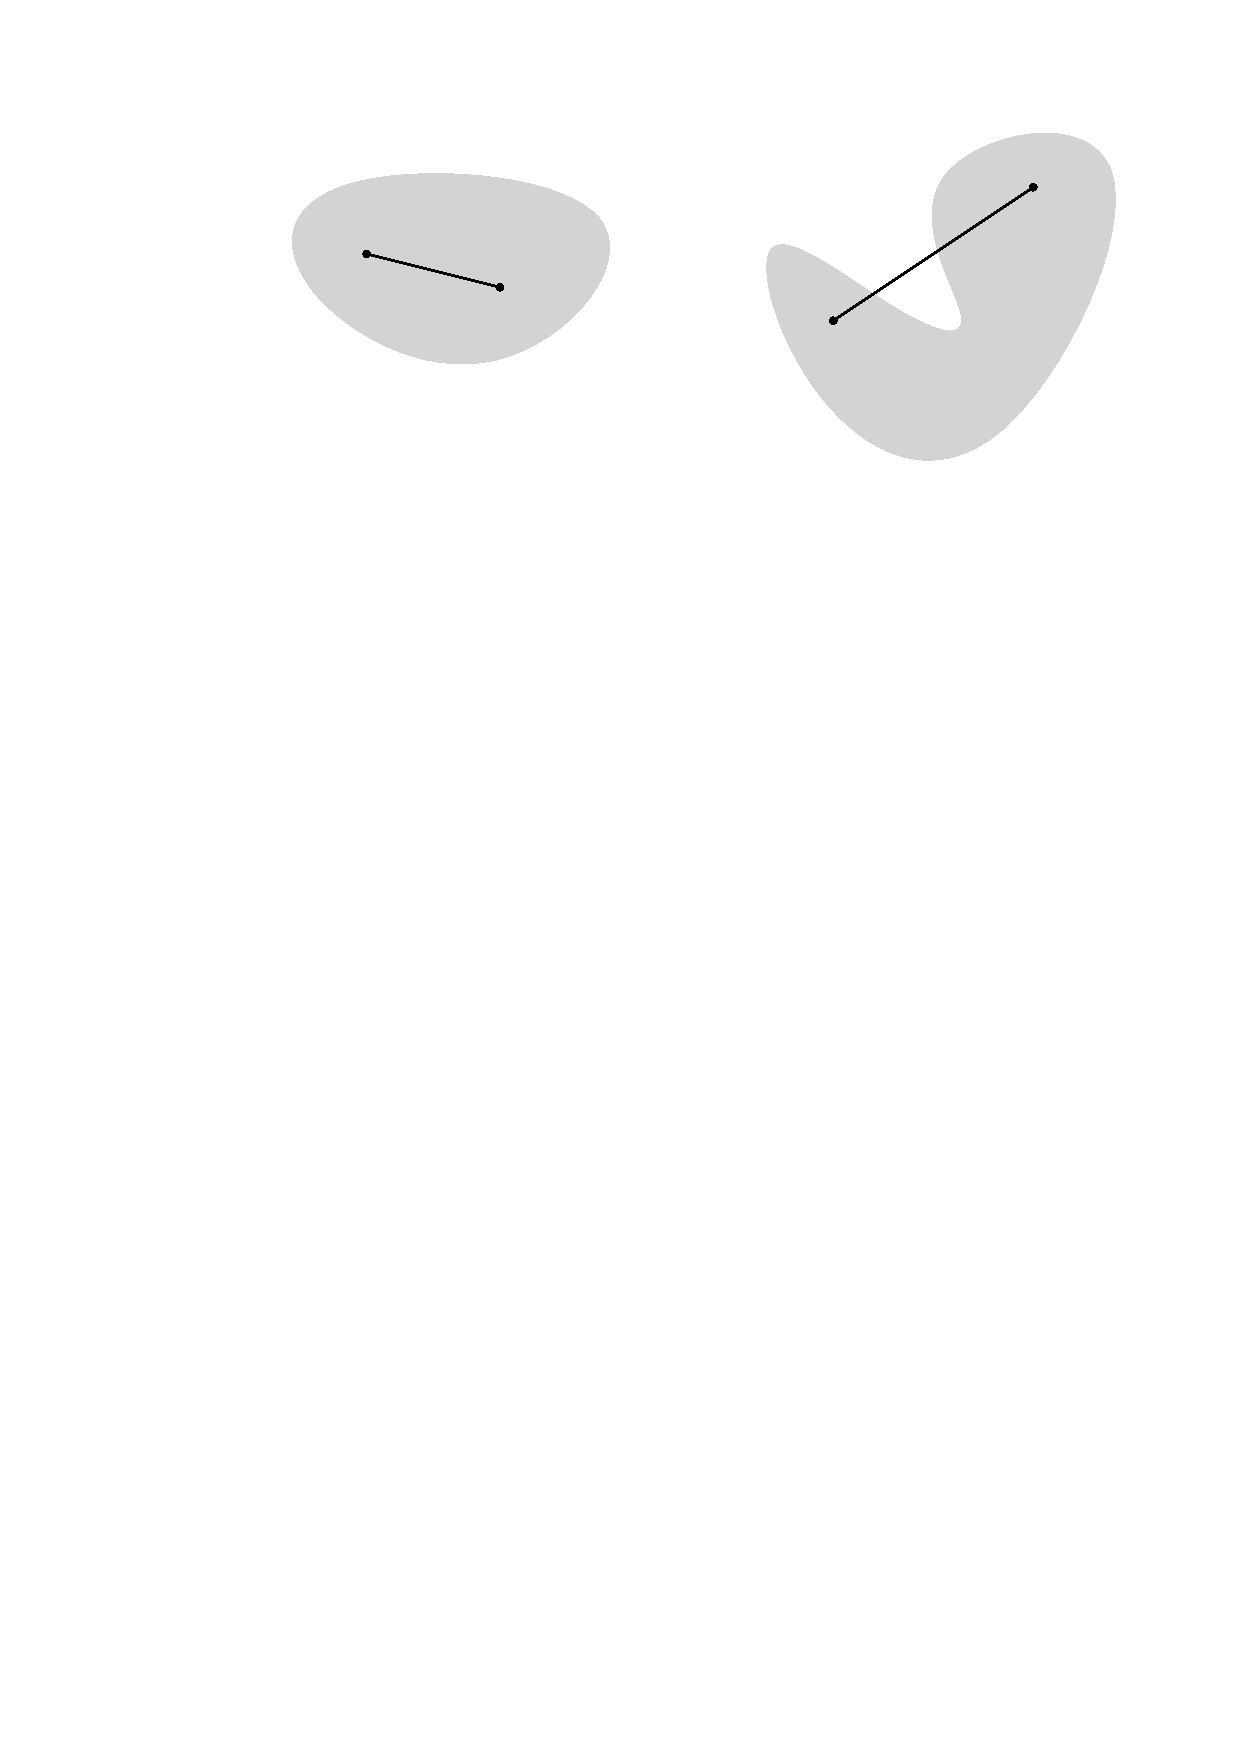
\includegraphics[height=3cm]{../figures/exconv.pdf} 



  
  \begin{columns}
    \begin{column}{.5\textwidth}
      
    \end{column}
    \begin{column}{.5\textwidth}
      
    \end{column}       
  \end{columns}
\end{frame}






\begin{frame}{Halfspaces}

  \begin{definition}    
    A \emph{halfspace} is a set  of the form
    \begin{displaymath}
  \{ x \in \R^n \colon a^Tx \leq \beta\}. 
\end{displaymath}

A \emph{hyperplane} is a set of the form 
\begin{displaymath}
  \{ x \in \R^n \colon a^Tx = \beta\}. 
\end{displaymath} 

  \end{definition}

  
  \begin{columns}
    \begin{column}{.5\textwidth}
      
    \end{column}
    \begin{column}{.5\textwidth}
      
    \end{column}       
  \end{columns}
\end{frame}





\begin{frame}{Halfspaces are convex}
\begin{lemma}
    A half-space is convex. 
  \end{lemma}
  \begin{columns}
    \begin{column}{.5\textwidth}
      
    \end{column}
    \begin{column}{.5\textwidth}
      
    \end{column}       
  \end{columns}
\end{frame}



\begin{frame}{}

  \begin{columns}
    \begin{column}{.5\textwidth}
      
    \end{column}
    \begin{column}{.5\textwidth}
      
    \end{column}       
  \end{columns}
\end{frame}




\begin{frame}{Intersections of convex sets}
\begin{lemma}
  \label{lem:1}
  Let $I$ be an index set and $C_i \subseteq \R^n$ be convex sets for
  each $i \in I$, then $\cap_{i \in I}C_i$ is a convex set.
\end{lemma}

\begin{corollary}
  A polyhedron is a convex set.  
\end{corollary}


\end{frame}





\begin{frame}{}

  \begin{columns}
    \begin{column}{.5\textwidth}
      
    \end{column}
    \begin{column}{.5\textwidth}
      
    \end{column}       
  \end{columns}
\end{frame}




\begin{frame}{Valid inequalities}


 



  \begin{columns}
    \begin{column}{.5\textwidth}
       \begin{definition}
    $a^Tx \leq \beta$ is \emph{valid} for $K \subseteq \R^n$ if for each $x^* \in K$:   $$a^Tx^* \leq \beta$$


    If in addition $(a^Tx = β) \cap K \neq\emptyset$, then
    $a^Tx\leq β$ is a \emph{supporting inequality} and $a^Tx = β$ is a
    \emph{supporting hyperplane}
\end{definition}

    \end{column}
    \begin{column}{.5\textwidth}
      
    \end{column}       
  \end{columns}
\end{frame}




\begin{frame}{Extreme points }



  
  
  \begin{columns}
    \begin{column}{.5\textwidth}
      \begin{definition}
  Let $K \subseteq \R^n$ be  convex. $x^* \in K$ is
 \emph{extreme point} or \emph{vertex} of $K$ if there exists a valid inequality $a^Tx \leq \beta$ of $K$ such that 
 \begin{displaymath}
   \{x^*\} = K \cap \{x \in \R^n \colon a^Tx = \beta\}.  
 \end{displaymath}
\end{definition}

    \end{column}
    \begin{column}{.5\textwidth}
      \centering
  
\includegraphics[height=3cm]{../figures/ExtremePoint.pdf} 



    \end{column}       
  \end{columns}
\end{frame}



\begin{frame}{Vertices of polyhedra -- algebraic characterization}

\begin{theorem}
  \label{thr:1}
  Let $P = \{x \in \R^n \colon Ax \leq b\}$ be a polyhedron. $x^* ∈ P$ is  extreme point iff  there is  sub-system $A'x \leq b'$ of  $Ax \leq b$  s.t. 
  \begin{enumerate}[i)]
  \item $x^*$ satisfies all inequalities of $A'x \leq b'$ with
    equality. \label{item:1}
  \item $A'$ has $n$ rows and $A'$ is non-singular. \label{item:2}
  \end{enumerate}  
\end{theorem}
{\small 
\begin{columns}
    \begin{column}{.5\textwidth}     
    \begin{displaymath}
      A =
      \begin{pmatrix}
        3 & 6 \\
        8 & 4 \\
        1 & 0 \\
        0 & 1 \\
        -1 & 0 \\
        0 & -1
      \end{pmatrix},
    \quad b = 
      \begin{pmatrix}
        30 \\ 44 \\ 5 \\ 4 \\ 0 \\ 0
      \end{pmatrix}:
    \end{displaymath}
 
    \end{column}
    \begin{column}{.5\textwidth}
      
      \begin{tikzpicture}[scale=.45]       
     
      \filldraw[fill=green!20,draw=green!20!](0,0) -- (0,4) -- (2,4) --
      (4,3) -- (5,1) -- (5,0) -- (0,0); 
      
      
      \draw [-,draw=gray] (7,1.5) -- (-1.5,5.75) ;
      \draw [-,draw=gray] (-1.5,4) -- (7,4) ;
      \draw [-,draw=gray] (5,-.5) -- (5,6) ;
      \draw [-,draw=gray] (2.5,6) -- (5.75,-.5) ;
      
      
          
      \draw[->] (-1.5,0) -- (8,0) node[below right] {$x_1$}; \draw[->]
      (0,-.5) -- (0,6) node[left] {$x_2$};
      
%      \draw[draw=blue] (-1.50000000000000,
%      7.40000000000000)node[left]{\small  
%        \color{blue}{$  \beta = 775$}} --
%      (8.37500000000000, -0.500000000000000) ; 
      
%      \filldraw [red] (4,3) circle (3pt)node[above right] {$(4,3)$};
      
          
%      \foreach \x in {1,...,7}
 %     \draw (\x cm,1pt) -- (\x cm,-1pt) node[anchor=north] {$\x$};
 %     \foreach \y in {1,...,5}
 %     \draw (1pt,\y cm) -- (-1pt,\y cm) node[anchor=east] {$\y$};     
    \end{tikzpicture} 


    \end{column}       
  \end{columns}}



  
  \begin{columns}
    \begin{column}{.5\textwidth}
      
    \end{column}
    \begin{column}{.5\textwidth}
      
    \end{column}       
  \end{columns}
\end{frame}








\begin{frame}{Optimal solutions and vertices}


\begin{theorem}
  \label{thr:2}
  If a linear program $\max\{c^Tx \colon x \in \R^n, \, Ax \leq b\}$
  is feasible and bounded and if $\rank(A) = n$, then the linear program has an optimal solution that is  an extreme point. 
\end{theorem}


  
  \begin{columns}
    \begin{column}{.5\textwidth}
      
    \end{column}
    \begin{column}{.5\textwidth}
      
    \end{column}       
  \end{columns}
\end{frame}







\begin{frame}{}

  \begin{columns}
    \begin{column}{.5\textwidth}
      
    \end{column}
    \begin{column}{.5\textwidth}
      
    \end{column}       
  \end{columns}
\end{frame}






\begin{frame}{Bounded LP has optimal solution}



\begin{corollary}
  \label{co:12}
  A linear program $\max \{ c^Tx : x ∈ ℝ^n, \, Ax ≤ b\}$ which is feasible and bounded has an optimal solution. 
\end{corollary}

  
  \begin{columns}
    \begin{column}{.5\textwidth}
      
    \end{column}
    \begin{column}{.5\textwidth}
      
    \end{column}       
  \end{columns}
\end{frame}






\begin{frame}{A first (inefficient) algorithm}

  Given $\max\{c^T x : x ∈ ℝ^n, \, Ax ≤b \}$  w.l.o.g. $\rank(A) =n$
  
  \begin{itemize}
  \item  Initialize $M = ∅$ 
  \item Enumerate all sets of $n$ row-vectors that are basis of $ℝ^n$
    \begin{itemize}
    \item    Solve $A'x = b'$ for corresponding system
    \item If for solution $x^*$: $Ax^* ≤ b$ then $M = M + x^*$      
    \end{itemize}
  \item Output point of  $M$  with largest objective function value 
  \end{itemize}

  \bigskip

  \begin{theorem}
    If LP is bounded then algorithm above computes optimal solution. 
  \end{theorem}


  \begin{alertblock}{We will see ...}
    ... we can do much better. 
  \end{alertblock}
\end{frame}





\begin{frame}{Bounded continuous functions}

\begin{theorem}

  Let $X\subseteq\setR^n$ be compact and $f: X \to \setR$ be continuous. Then $f$ is
  bounded and there exist
  points $x_1,x_2 \in X$ with $f(x_1) = \sup\{ f(x) \colon  x \in X\}$ and
  $f(x_2) = \inf \{ f(x) \colon x \in X\}$. 
\end{theorem}
  
  \begin{columns}
    \begin{column}{.5\textwidth}
      
    \end{column}
    \begin{column}{.5\textwidth}
      
    \end{column}       
  \end{columns}
\end{frame}







\begin{frame}{Separation theorem}

\begin{theorem}

  Let $K\subseteq\setR^n$ be a closed  convex set and $x^* \in \setR^n \setminus K$, then there
  exists an inequality $a^Tx ≤ \beta$ such that $a^T y < \beta$ holds for all
  $y \in K$ and $a^Tx^*>\beta$. 
\end{theorem}

  \begin{columns}
    \begin{column}{.5\textwidth}
      
    \end{column}
    \begin{column}{.5\textwidth}
      
    \end{column}       
  \end{columns}
\end{frame}






\begin{frame}{}

  \begin{columns}
    \begin{column}{.5\textwidth}
      
    \end{column}
    \begin{column}{.5\textwidth}
      
    \end{column}       
  \end{columns}
\end{frame}






\begin{frame}{Farkas' Lemma -- Version 1}



\begin{theorem}[Farkas' lemma]
  \label{conv:thr:12}
  Let $A \in \setR^{m\times n}$ be a matrix and $b \in \setR^m$ be a vector. The
  system $Ax = b, \,x\geq0$ has a solution if and only if for all $\lambda \in
  \setR^m$ with $\lambda^TA\geq0$ one has $\lambda^Tb \geq0$.  
\end{theorem}
  
  \begin{columns}
    \begin{column}{.5\textwidth}
      
    \end{column}
    \begin{column}{.5\textwidth}
      
    \end{column}       
  \end{columns}
\end{frame}





\begin{frame}{}

  \begin{columns}
    \begin{column}{.5\textwidth}
      
    \end{column}
    \begin{column}{.5\textwidth}
       
    \end{column}       
  \end{columns}
\end{frame}






\begin{frame}{Farkas' Lemma -- Version 2}

\begin{theorem}[Farkas' lemma]
  \label{conv:thr:12}
  Let $A \in \setR^{m\times n}$ be a matrix and $b \in \setR^m$ be a vector. The
  system $Ax ≤ b$ has a solution if and only if for all $\lambda \in
  \setR_{≥0}^m$ with $\lambda^TA = 0$ one has $\lambda^Tb \geq0$.  
\end{theorem}

\bigskip 
Exercise! 
 
\end{frame}





%%% Local Variables:
%%% mode: LaTeX
%%% TeX-master: "Slides"
%%% End:

 
\end{document}


%%%Local Variables:
%%% mode: latex
%%% TeX-master: t
%%% TeX-engine: xetex
%%% End:
